\documentclass[preprint]{sigplanconf}
\usepackage{cleveref,amsmath,chngcntr}
\usepackage{textcomp} % for tilde
\usepackage{paralist} % for in-paragraph lists
\usepackage{url}
\usepackage{graphicx}
\usepackage{multicol,multirow}
\usepackage{tabularx}

% For drawing FSMs
%\usepackage{tikz}
%\usetikzlibrary{arrows,automata}

% Used for code snippets
\usepackage{listings,courier}
\usepackage{subfig,epsfig}
\DeclareCaptionType{copyrightbox}
\usepackage{epsfig}


% Settings on code listings.
\lstset{language=C,
		xleftmargin=0pt,
		xrightmargin=0pt,
		framexbottommargin=0pt,
        framextopmargin=0pt,
        framesep=0pt}
\usepackage{enumitem}

% Add listing language for assembly
\lstdefinelanguage
   [x64]{Assembler}     % add a "x64" dialect of Assembler
   [x86masm]{Assembler} % based on the "x86masm" dialect
   % with these extra keywords:
   {morekeywords={CDQE,CQO,CMPSQ,CMPXCHG16B,JRCXZ,LODSQ,MOVSXD, %
                  POPFQ,PUSHFQ,SCASQ,STOSQ,IRETQ,RDTSCP,SWAPGS, %
                  rax,rdx,rcx,rbx,rsi,rdi,rsp,rbp, %
                  r8,r8d,r8w,r8b,r9,r9d,r9w,r9b}} % etc.


% For leaving some comments in the draft.
\newcommand{\comment}[1]{}

% For writing Granary tool names.
\newcommand{\toolname}[1]{{\scshape #1}}

% Customize cleverref
\crefname{section}{Section}{Sections}


\begin{document}

%make title bold and 14 pt font (Latex default is non-bold, 16 pt)
\title{Fast and Flexible Binary Instrumentation for the Kernel}

%for single author (just remove % characters)
\authorinfo{Peter Goodman \and Angela Demke Brown \and Ashvin Goel}
{University of Toronto}{}
% end authorinfo

\maketitle
\subsection*{Abstract}
%Kernel modules extend the functionality of operating systems. They represent the bulk of new kernel code in development and contain the majority of new kernel bugs. Unfortunately, analyzing and debugging modules is very challenging. Static analysis of module source code is difficult because of the tight interaction between modules and the kernel. Some modules, however, are only distributed in a binary format, which makes static analysis intractable. Existing dynamic analysis tools capable of instrumenting modules are not suited toward module analysis. They either impose unnecessary performance overheads, lack flexibility and are too coarse-grained, or do not provide a means of understanding the ``big picture'' view of what an arbitrary module does as it executes.

%We created Granary to address the challenges of module analysis. Granary is a framework for creating flexible and efficient tools that analyze or debug arbitrary, binary Linux kernel modules. Granary uses dynamic binary translation to dynamically rewrite and comprehensively instrument kernel modules. Granary makes it easy to create flexible tools by supporting context-aware runtime code specialization, and by integrating high-level static analysis information with low-level instruction manipulation. Module analysis tools built on Granary are efficient because of Granary's adoption of a relaxed transparency model, and because of Granary's ability to instrument module code without imposing overhead on non-module kernel code.

\section{Introduction}\label{sec:intro}

Granary is a framework for creating flexible and efficient tools that instrument the Linux kernel. Granary's key novelty is its \emph{runtime code specialization} feature, which enables tools to decide what code to instrument, and how to instrument that code. Flexible specialization allows tools to be picky about instrumentation. For example, a tool can choose to instrument every load and store operation, but only inside nested critical sections that are executing in module code. Granary's runtime code specialization feature addresses two limitations of existing kernel analysis systems: \begin{inparaenum}[i)]
	\item they have focused on instrumenting all code \cite{DRK,btkernel,QEMU}; and
	\item they can only instrument code using a single policy.
\end{inparaenum} 

%Operating system (OS) kernels present an apparently insane environment for a transparent binary instrumentation framework.  For example, hardware interrupts can redirect control flow at any instruction, and interrupt delivery cannot be delayed past the execution of memory instructions that might alter the interrupt delivery state~\cite{DRK}. Preserving interrupt transparency, however, requires that interrupts be delayed until the end of any injected instrumentation instructions.  Together, these requirements make it very difficult to write instrumentation tools.  The insane environment of OS kernels also creates several opportunities for analysis tools. For example, interrupts can be ``tamed'' and put to new uses; privileged hardware features can be used; and the kernel ABI and source code can be relied upon to be a good predictor of module behavior at the kernel/module boundary. We also found that the kernel is largely insensitive to transparency issues, allowing us to relax transparency in exchange for both improved performance and greater visibility into the execution of instrumented code.  This increased visibility is particularly important for analysis and debugging tools.

%The challenges and opportunities of the kernel environment motivated the creation of Granary. Granary is a new binary instrumentation framework for the Linux kernel environment, designed specifically for analyzing kernel modules. Granary targets modules because they represent the bulk of new bugs and new code in development in the Linux kernel \cite{FaultsInLinux}. Granary allows developers to create flexible and dynamic analysis tools for arbitrary Linux kernel module binaries. Granary has two main goals: \begin{inparaenum}[i)]
%	\item make it easy to create efficient, low-level analysis tools; and
%	\item provide high-level static analysis information to the analysis tools.
%\end{inparaenum} Granary achieves the first goal by using dynamic binary translation (DBT) to provide low-level access to instructions, memory, and interrupts. Granary achieves the second goal by giving tools direct access to the results of its own static analysis of the Linux kernel source code. By meeting these goals, Granary tools are able to do things like  figure out which data structure fields are associated with each memory access.

%Granary addresses three limitations of existing program analysis systems: \begin{inparaenum}[i)]
%	\item they have focused on instrumenting all code \cite{DRK,btkernel,QEMU};
%	\item they do not allow for flexible runtime code specialization; and
%	\item they do not provide static type information to the instrumented code.
%\end{inparaenum} 

Instrumenting all code (e.g., the whole kernel) imposes unnecessary performance overheads when only a subset of the code is being analyzed (e.g., modules, functions). In practice, we would like to target instrumentation at specific code for efficiency, while also allowing rich and detailed instrumentation of the targeted code. Limiting the scope of what is instrumented is  important because the overhead introduced by using runtime code instrumentation is usually dominated by the instrumentation itself and not the baseline overhead of the runtime system supporting that instrumentation. Also, specializing based on what is instrumented allows instrumentation tools to avoid unnecessary filtering. That is, if one wants to instrument RCU read-side and write-side critical sections, as is the case with Granary's \toolname{RCUdbg} tool, then instrumenting all code just to filter out / find those sections is wasteful.

%This requirement motivates the design of \emph{mixed-mode execution}, which allows Granary tools to instrument only specific code while the majority of code executes with zero overhead. 

%This is challenging because Granary must be comprehensive: all code that is meant to be instrumented should be instrumented. In other words, relinquishing control to execute kernel code natively must not cause Granary to miss the execution of any module code.

Another limitation of existing systems is that they are unable to perform efficient runtime code specialization, i.e. they are unable to change how code is instrumented based on the context in which that code will run. This is unfortunate because it means that tools wanting to instrument code differently must create their own solution that works around this deficiency of existing systems. A typical solution is for tools to generate as many instrumented versions of the code as there are execution contexts. When instrumented code is  executing, runtime checks query some thread-private or CPU-private state, and jump to the correct version of the code for the current context. Runtime checks of this form are inefficient, and generating many versions of the code introduces bloat. The machinery needed to multiplex between different versions of instrumented code is also orthogonal to the goals of the instrumentation tool, thus distracting tool-developers from their primary objectives.

%Using an existing system, 
% get around the problem of needing different instrumentation in different contexts, existing systems need to create as many versions of the code as there are contexts. Runtime checks must also be inserted into the code that coordinate with the runtime to track and detect the current execution context and jump to the correct version of the code. Runtime checks and state tracking impose unnecessary complications to tool-authors. The added code needed to query the current context and switch to a different version of the instrumentation is code that is not actively achieving the primary goal of the tool, and is instead making up for a defeciency in the runtime system.  
%are orthogonal to the main goals of an analysis tool:
% Aside from the additional ineffeciency of these runtime checks, there is also the 
% However, generating many differently instrumented versions of the code introduces bloat, especially when not all versions are well exercised. Also, generating many different versions of the code introduces state tracking and switching costs.
% This imposes unnecessary performance overheads because of the need to additional instrumentation that is unrelated to 
% due to having to perform runtime detection and swichting
% to the right version of the code for every basic block or every instruction.
% according to \emph{all} contexts. Instrumenting code according to all contexts imposes unnecessary performance overheads and requires state tracking.
%,  dynamically tracking the current context, and dynamically choosing which 
% commit to instrumenting code to handle \emph{all} contexts. For example, if 

One example of a tool that uses runtime code specialization is Granary's Read-Copy-Update (RCU) debugging tool, \toolname{RCUdbg}. \toolname{RCUdbg} catches bugs related to invalid uses of RCU-protected pointers (\Cref{sec:rcudbg}). \toolname{RCUdbg} distinguishes between two kinds of RCU-protected pointers (reader-side and writer-side) and plain old pointers, and three execution contexts (inside of a read-side critical section, inside of a write-side critical section, and in non-RCU-related code). The actions taken when a pointer is de-referenced varies depending on the kind of pointer and the execution context. Code executing in read-side critical sections is specialized to enforce that only plain-old and read-side pointers are accessed, and that all accesses through read-side pointers are memory reads. Write-side critical sections are specialized in a similar way.

%There are similar checks for write-side pointers in write-side critical sections.
% The instrumentation performed inside of read- and write-side critical sections is heavy weight, while code running in the third execution context can either run with lightweight or no instrumentation.
%RCUdbg distinguishes between RCU-protected pointers and plain old pointers. There are two kinds of RCU-protected pointer (read-only, and read/write), and every access to an RCU-protected pointer is checked. The checks performed on an access to an RCU-protected pointer are context-specific. That is, a read-only pointer can only be read from within an RCU read-side critical section. Read/write pointers have similar restrictions. RCUdbg needs to know in which context some code is executing, i.e. in a read-side or write-side critical section, or outside of all critical section, and change instrumentation to check for different kinds of bugs based on the context.
%A read/write pointer has different restrictions. In read-side critical sections, a read/write pointer can only be accessed by means of a special API function. In write-side critical sections, a read/write pointer can only be written to 
% One kind of RCU-protected pointer can be read from within ``RCU read-side critical sections", while another kind can (almost) arbitrarily accessed, but only inside of an ``RCU write-side critical section". Outside of these two kinds of sections, accessing RCU-protected pointers is illegal. The distinction between different contexts of code (read-side, write-side, outside), and different kins of pointers makes
%Creating a tool to catch these kinds of bugs with an existing DBT system would be difficult because that tool would need to  
%For example, Granary's Read-Copy-Update (RCU) debugging tool, \toolname{RCUdbg}, specializes instrumentation at different stages of use of the RCU synchronization API. Correct usage of the RCU API allows programmers to create scalable, shared data structures that permit concurrent access and modification. The ``trick" of RCU is that readers might not see the latest write to the data structure, and writers must synchronize to modify the data structure. \toolname{RCUdbg} distinguishes between code executing inside \emph{read-side} and \emph{write-side} critical sections, and instruments each code context differently. In read-side critical sections, \toolname{RCUdbg} detects bugs when readers access potentially non-existent data, do not the correct accessor API, or attempt to write to shared data. In write-side critical sections, \toolname{RCUdbg} detects when writers write to shared data without using the correct API. 
%In reader-side code
%For example, Granary has a tool that  dynamically constructs inter- and intra-procedural control flow graphs (CFGs). The outputs of this tool enable Granary to do better runtime register allocation, which improves tool efficiency. Part of building CFGs requires tracking whether or not a given basic block is the entrypoint to a function. This is challenging with existing DBT systems because some optimized functions will re-execute their first basic block, which might incorrectly appear as new function calls in the CFGs. Granary solves this problem using demand-based runtime code specialization: every entrypoint basic block is instrumented in one way, and later re-executions of any entrypoint basic blocks are specialized and instrumented in another way.

The \toolname{RCUdbg} tool is an example of \emph{context-driven code specialization}: code executing inside of a read-side critical section is instrumented differently from code executing inside of a write-side critical section, and code executing outside of both contexts runs natively or with lightweight instrumentation. Achieving this level of specialization using and existing system requires complicated runtime state management and checks to switch between different versions of the code. With Granary, a tool like \toolname{RCUdbg} can specialize code using instrumentation policies. An instrumentation policy is a function that names an execution context and decides how to instrument instructions that will execute within that context. When a policy is used to instrument a sequence of instructions (called a basic block), a new version of the basic block is generated and cached. 

\toolname{RCUdbg} defines three policies, and declares transitions between these policies when control flows in and out of RCU read- and write-side critical sections. When a function like \texttt{memset} is invoked in one context, the policy associated with that context is used to generate an instrumented version of \texttt{memset} for that context. If, for example, \texttt{memset} is never invoked within a read-side critical section, then \texttt{memset}'s code will never be specialized to perform the heavyweight checks needed to detect RCU-protected pointer misuses in this context. Similarly, if \texttt{memset} is executed both in a write-side critical section and outside of any RCU-related code, then two differently instrumented versions of \texttt{memset} will be generated.

The key insight of Granary's approach to runtime code specialization is that code versioning is a context-tracking mechanism. That is, if an instruction from a basic block instrumented by \toolname{RCUdbg}'s read-side critical section policy is being executed, then the current thread must be executing inside of a read-side critical section. Similarly, if the read-side policy is used to instrument a basic block, then \texttt{RCUdbg} knows at instrumentation time\footnote{Instrumentation time is analogous to ``compile time", in that a policy is generally used to instrument a basic block of code once, and then that basic block may be executed many times.} that this basic block will only execute within a read-side critical section. If the basic block contains a \texttt{call} to the \texttt{memset} function, then \texttt{memset} is also known to execute within a read-side critical section because it does not terminate a read-side critical section. By deciding which version of \texttt{memset} to execute at instrumentation time, \toolname{RCUdbg} avoids expensive runtime checks that other systems impose in order to achieve similar kinds of specialization. \toolname{RCUdbg} can specify that \texttt{memset} will also execute within a read-side critical section by telling Granary that it should use the read-side critical section policy to instrument \texttt{memset}. 

%Granary records 
%Policy information is recorded inside of Granary's 

% instruction by telling Granary what policy to use to instrument the code 
%, and when the \texttt{call} is eventually executed, 
%This simplifies tool creation becase 
%By propagating policy information through control-flow transferring instructions, 
%Therefore, we can know at translation and instrumentation time that
% No additional state needs to be maintained by \texttt{RCUdbg} to determine which version of the basic block to execute.
%Any control-flow instructions the transfer control to other basic blocks that aren't the \texttt{rcu\_read\_unlock} function must also 
%That is, the failure of existing systems is that they have no built-in support for maintaining multiple versions of code. Tools built on existing systems must emulate versioning by duplicating their instrumentation for each desired version, and add code that executes the right version at the right time.  
%, as would be done using existing systems, 
%What makes Granary's runtime code specialization efficient is that it ties into Granary's \texttt{just-in-time} instrumentation model. That is, Granary only instruments code that will execute. Code that never executes is neither translated nor instrumented. Also, only one version of a basic block is generated at a time. Therefore, even though \toolname{RCUdbg} defines three policies, only
%If some native code is about to execute, then Granary will only instrument it with the policy associated with 
%, and an instrumentation policy is only applied to code if that code will execute within the context associated with that context.
%defines three different instrumentation policies--one for each execution context--and declares switches 
% instrumentation policies to 
%only needs to define three instrumentation policies (one for each execution context), and declare 
%different versions of the code are generated \emph{just-in-time}. Therefore, if the \texttt{memset} function is never executed inside of a read-side critical section, then \texttt{memset}'s code will never be specialized to perform the heavyweight checks needed to detect RCU-protected pointer misuses in this context. Similarly, if \texttt{memset} is executed both in a write-side critical section and outside of any RCU-related code, then two differently instrumented versions of \texttt{memset} will be generated. 
%However, unlike other systems, no runtime check that chooses to dispatch to one version of \texttt{memset} or another depending on the runtime context. Instead, 
% if some code never executes in a particular context, then Granary will not generate an instrumented version of that code for that context.  The second benefit of this approach is that it is stateless, and requires no runtime checks to switch between different versions of the code depending on the execution context. 
%Granary tracks the current execution context with zero runtime overhead by 
%In a Granary tool, each tracked execution context is associated with its own instrumentation policy. An instrumentation policy decides how to instrument code that will execute within the associated context. 
%Different versions of the code are instrumented \emph{just-in-time}. That is, there will 
%Granary is able to track execution contexts because it explicitly maintains policy information in translated basic blocks. This avoids typical poblems with tracking context in just-in-time DBT systems (e.g., maintaining runtime context-tracking state, reentrancy, and the inability to predict later execution contexts at translation time).
% In the previous example, executing code is classified into two contexts: entrypoint and non-entrypoint basic blocks.  In the case of our CFG tool, two policies track the two execution contexts: $P_{\mathit{call\_entry}}$ and $P_{\mathit{after\_entry}}$. $P_{\mathit{call\_entry}}$ applies to the first execution of the first basic block of each function, and connects functions in the inter-procedural CFG.  $P_{\mathit{after\_entry}}$ applies to all other executed basic blocks within each function, including re-executions of the first basic block. $P_{\mathit{after\_entry}}$ connects basic blocks in the intra-procedural CFG. 
%Finally, an important missing feature of existing low-level instrumentation systems is the ``big picture'' view that one gets from static analysis information. Similarly, static analysis tools lack access to instructions, memory, and processor-specific behaviors that are only available to low-level runtime instrumentation tools. Existing mixed static/dynamic analysis tools \cite{NaCl,AddressSanitizer,ThreadSanitizer} appear to get the best of both worlds, but sacrifice on runtime flexibility by committing to a single instrumentation policy at a program's compile time. The benefits of high-level static analysis motivated its inclusion into Granary using a technique we call \emph{reifying instrumentation}. Granary statically analyzes the Linux kernel source code to bootstrap learning about  the interfaces that enable modules and the kernel to interact. Granary exposes this information to instrumentation tools in the form of type and function \emph{wrappers}. Tools can use wrappers to apply context-specific policies when instrumenting module code as well as to inspect and manipulate parts of kernel/module memory in a type-safe way.
%For example, we are actively developing a tool that uses static type information to learn about all the fields of all kernel data structures that are read from or written to by modules. This information allows us to model things like how a typical file system operates on kernel data structures in the process of opening a file. From these models, we can construct behavioral patterns about how modules use kernel data structures and functions. These patterns can be used to classify modules \cite{DeviceDriverClassification} and identify spurious behavior \cite{LXFI}.

The rest of the paper describes Granary in more detail. \Cref{sec:dbt} describes how Granary is implemented, \Cref{sec:what} describes how a Granary tool can choose to instrument only specific code, \Cref{sec:how} describes how Granary change the policy used to instrument code, etc.

% \Cref{sec:modes} describes how to efficiently implement mixed-mode execution. \Cref{sec:policies} describes a new method for dynamically changing how code is instrumented. \Cref{sec:reify} describes how to integrate static analysis information into a DBT system. Finally, \Cref{sec:eval} evaluates Granary's performance.

\section{Dynamic Binary Translation}\label{sec:dbt}

Granary uses dynamic binary translation (DBT) to instrument the Linux kernel. DBT is used for emulation \cite{QEMU}, runtime optimization \cite{DynamoRIOOptimization}, and runtime instrumentation (analysis \cite{DynamoRIO, DRK, btkernel, ProfilingSimics}, security \cite{Vx32,NaCl,ProgramShepherding}, and debugging \cite{Valgrind}). We chose DBT because \begin{inparaenum}[i)]
	\item static binary analysis tools are unable to cope with \texttt{x86}'s mix of variably-sized instructions and data; 
	\item some kernel code is only distributed in a binary format (e.g. proprietary device drivers); and
	\item virtualization-based approaches are unable to analyze non-virtualizable device drivers \cite{DRK}.
\end{inparaenum}

%Granary translates and instruments code at one of three default granularities: kernel, module, and function (also called probe-based instrumentation). 
%
%At runtime, the granularity of instrumentation can be altered based on the execution context. For example, a tool analyzing modules for bugs can choose not to instrument a particular function (e.g. whitelist the function) if that function is known to not contain bugs, or known to generate many false-positives.
%
%\paragraph{Kernel}
%Granary interposes on the system call and interrupt entrypoints, located in the x86-64 \texttt{MSR\_LSTAR} model-specific register and interrupt descriptor table (IDT), respectively. 
%
%\paragraph{Module}
%
%
%\paragraph{Function}
%
%Granary can interpose on the execution of specific kernel functions in three ways:
%\begin{enumerate}
%	\item {\bf Wrapping:} Granary can substitute the execution of a kernel function when that function is invoked from instrumented code. A different function can be substituted depending on the context from which the original function is invoked (instrumented kernel code, instrumented module code). We call this type of interposition ``wrapping'' because it is commonly used to inspect the substituted function's arguments and return value, while still invoking the original function.
%	\item {\bf Substituting:} Granary can substitutes the execution of a kernel function, even when that function is executed by native kernel code. This is useful when tools only instrument part of the kernel (e.g. modules or functions) but require visibility on specific kernel events happening outside of the instrumented code (e.g. particular memory allocations).
%	\item {\bf Instrumented Wrapping/Substituting:} Granary can optionally instrument wrapped or substituted code. This is useful when tools want to observe function arguments/return values using high-level C/C++ code, but where that function must be instrumented for visibility.
%\end{enumerate}

Granary translates and instruments kernel binaries one basic block at a time. In Granary, a basic block is a sequence of x86-64 instructions ending in a conditional branch, \texttt{ret}, or a \texttt{jmp} instruction. Unlike DRK and DynamoRIO, Granary does not terminate basic blocks at \texttt{call} instructions. This enables longer basic blocks and native-like proceccor return address prediction, but makes Granary non-transparent (\Cref{sec:transparency}). Entrypoint basic blocks (e.g. interrupt vectors, system call entrypoints, module initializers) are translated ahead-of-time, and all other basic blocks are translated just-in-time (JIT) as execution ``discovers'' them.

Translated basic blocks are linked together and stored in a \emph{code cache}. Basic blocks are indexed by $(pc, policy)$ pairs, where $pc$ is the native program counter associated with the beginning of the basic block's instructions, and $policy$ is the instrumentation policy used to instrument the native instructions starting at $pc$. The index is maintained by a globally accessible hash table.

Granary's just-in-time translation approach means that code executing from the code cache may yield control to Granary to request the address of the next basic block to execute. When instrumented code yields to Granary, a ``context switch'' occurs that transfers execution to a CPU-private stack where Granary operates. Granary operates on a CPU-private stack for two reasons. First, if Granary did not switch stacks, then context switches into Granary risk overflowing the runtime call stack. This can happen because kernel stacks are typically small (4K to 8K in size), and because a context switch could happen when the native stack is nearly exhausted. Second, on an SMP, multiple processors can simultaneously execute Granary code (e.g. to translate code that will later execute). In such cases, Granary depends on CPU-private data structures to avoid contention, and the stack is one such data structure. A context-switch back to the code cache occurs when the next basic block has been found or translated. At this point, instrumented execution continues. Similar to other DBT systems, Granary uses caching and hot code patching to reduce the number of context switches. In our experience, kernel code stabilizes very quickly: context switches stop happening after the first few seconds of translation.

%Granary code executes with interrupts disabled and depends on CPU-private data to avo
%Granary's translation mechanism depends on CPU-private data to avoid contention when two or more processors simultaneously execute Granary code.
%because kernel stacks are typically small (4K to 8K in size), and because context-switches into Granary can occur at arbitrary program points, Granary cannot risk 
%and a context switch into Granary might occur at any point. If most of the stack is already used by current thread before it yields control to Granary then 

\subsection{Basic Block Meta-Data}\label{sec:metadata}

Associated with each basic block is meta-data that describes the basic block. Basic block meta-data includes: \begin{itemize}
	\item The length in bytes of the original and translated basic blocks, and the address of the first instruction in the original basic block and the instrumented basic block. This information helps provide a rich debugging interface for instrumentation tool authors. Granary is unique among DBT tools in that the debugging experience is actually pleasant. For example, Granary has a built-in debugging mechanism for stepping back in time through previously executed basic blocks, as well as querying past register state.
	\item Linux kernel-specific exception table meta-data about instructions contained within the current basic block. This kernel-specific meta-data is used by Granary to implement transparent page fault exception handling (\Cref{sec:interrupt_return_address_transparency}).
	\item Ranges of instructions that must be executed atomically. Granary uses this information to implement selective interrupt delaying (\Cref{sec:interrupt_delay}).
	\item The allocator used to allocate the instructions of the basic block. Granary uses this information to implement its trace-allocation optimization (\Cref{sec:trace_alloc}).
	\item The instrumentation policy used to instrument the basic block. Granary uses this information to allow instrumentation tools to define policy-specific interrupt handling routines. For example, \toolname{RCUdbg} implements a read-side policy-specific interrupt handling routine that reports an error if a code executing within a read-side critical section is interrupted (\Cref{sec:rcudbg}).
\end{itemize} %
%Granary uses basic block meta-data for trace allocation (\Cref{sec:trace_alloc}), interrupt delaying (\Cref{sec:interrupt_delay}), and policy-specific interrupt handling.

Basic block meta-data can be also be extended by instrumentation tools. This makes developing instrumentation tools that record per-basic block statistics very easy to make. For example, Granary's control-flow graph tool, \toolname{cfg}, extends the basic block meta-data to track per-block and per-edge execution counts (\Cref{sec:cfg}). This data is useful because it provides precise code coverage information (block and branch coverage), as well as useful data for profile-guided optimization. This meta-data is specified by \toolname{cfg} and automatically allocated for \toolname{cfg} by Granary. 

%Basic block meta-data can also contain Granary's intermediate representation for x86-64 instructions. This is a unique feature that enables instrumentation tools to implement their own form of hot-code patching (among other things), as the intermediate representation remains tied to an emitted x86-64 instruction once the block is committed to the code cache.

%Unlike any other instrumentation tool, Granary allows the x86-64 instruction intermediate representation 

%Another 

%novelty of Granary is that basic block meta-data enables a good 

%Basic block meta-data is queried and extended by Granary instrumentation tools.



%// TODO!

%Block meta-data is also queried by interrupt handlers when deciding how to handle interrupts and exceptions in instrumented code, and by debuggers (e.g., \texttt{gdb}) to give contextual information about a translated basic block. This enables policy-specific interrupt handling. That is, when a basic block instrumented by a specific policy is interrupted, that policy can choose how to handle the interrupt. For example, Granary's address watchpoints framework can instrument code using a lightweight, \toolname{null} instrumentation.

\subsection{Transparency}\label{sec:transparency}
An instrumentation system is transparent if, given the same inputs, the instrumented and uninstrumented versions of a program behave in the same way \cite{Transparency}. Granary includes configurable levels of transparency to address the trade-off between transparency and overhead. By default, Granary uses a relaxed transparency model for efficiency, flexibility and increased visibility, but if instrumentation for some module requires transparency then it can be enabled at the cost of increased overheads and decreased visibility. By default, Granary exposes the following two artifacts: code cache addresses as function and interrupt return addresses.

\subsubsection{Function return addresses}\label{sec:return_address_transparency}
Unlike most DBT frameworks, Granary's basic blocks do not terminate at \texttt{call} instructions. This exposes code cache addresses to instrumented module code in the form of return addresses stored on the runtime call stack. The benefit of including \texttt{call} instructions are: \begin{enumerate}

	\item {\bf Zero overhead procedure returns.} Unlike Granary, DRK emulates procedure calls and returns. DRK emulates \texttt{call} instructions by pushing the intended native return address onto the runtime call stack, followed by a direct direct jump to the next (instrumented) basic block \cite{DRK}. This approach enables return address transparency, but introduces additional overheads on procedure returns, which must do costly indirect branch lookups to find the intended return target. 

Btkernel's approach is similar in spirit to Granary's; however, btkernel ends basic blocks at \texttt{call} instructions. This introduces unnecessary control-flow on the return path from procedures. That is, btkernel's ``call/ret optimization" ostensibly enables zero-overhead procedure returns by leaving \texttt{ret} instructions as-is; however, the benefits are more apparent than real. To transfer control to the next logical basic block after a procedure return, btkernel's \texttt{ret}s first transfer control to the end of the basic block that performed the \texttt{call}, and then \texttt{jmp} to the next basic block. Granary avoids this unnecessary \texttt{jmp} because basic blocks do not end at \texttt{call} instructions.
	
In some cases, emulating DRK's return-address lookup mechanism is desirable. For example, if Granary attaches while some program's execution is underway (and so the runtime call stack contains native return addresses), then a direct \texttt{ret} back to one of the native return addresses might be undesirable (e.g. if the tool wants comprehensive instrumentation of all code). In such cases, a tool can partially specialize instrumentation according to whether or not the return address might be in the code cache. Partial specialization is enabled by \emph{policy properties}, which are transparently inherited along with normal instrumentation policy information. In this case, the policy property can be used to tell Granary to emulate \texttt{ret} instructions when the return address is potentially a native address, and directly \texttt{ret} when the return address is known to be in the code cache.\footnote{This feature is used when Granary is configured to instrument user space programs. User space Granary depends on the Linux dynamic loader to inject Granary into a running process. When injected, a Granary takeover function is executed on an already active native runtime call stack. Granary's takeover procedure transparently emulates returns, thus taking over the previously fully-native call stack. This feature allows instrumentation tools to focus on their particular objectives and not the intricacies of thread takeover.}

%performing a \texttt{ret} requires an additional \texttt{jmp} to 
%Neither of DRK's nor btkernel's approaches enable native-like return address prediction by the CPU.
%and then jumping to the next basic block. This in turn . Btkernel's approach to procedure calls introduces similar inefficiencies, despite the fact that does not provide return address transparency, because it also emulates procedure calls, but by manually pushing the instrumented return address onto the stack instead of the native one.
%Granary's approach improves on DRK and btkernel by allowing 
%Better return-address prediction by the processor.

	\item {\bf Improved visibility.} Not ending basic blocks on \texttt{call} instructions results in longer basic blocks, which in turn provide additional visibility to tools at instrumentation time into what will be executed by the current thread. \toolname{RCUdbg} benefits from this additional visibility because it can observe the end of read-side critical sections (\texttt{call}s to \texttt{rcu\_read\_unlock}), and optimistically assume that functions executing before the read-side critical section ends will execute within the read-side critical section.

	%longer basic blocks, which provide more code visibility to instrumentation tools at instrumentation time.
\end{enumerate}

\subsubsection{Interrupt return addresses}\label{sec:interrupt_return_address_transparency}
Kernel interrupts are not sensitive to return addresses and hence relaxing return address transparency has no effect on interrupts. A special case arises for page fault exceptions that occur within specific kernel functions that access user space data \cite{btkernel}. The Linux kernel records ranges of code addresses that are permitted to fault in an ``exception table'' data structure, and on a page fault exception, checks if the exception return address belongs to one of the pre-defined ranges. Granary records any exception table entries as part of each basic block's meta-data, so that a page fault in a basic block can be mapped to the correct native faulting program counter.

%\paragraph{Module function wrappers} Granary does not maintain transparency when its type wrappers replace pointers to module functions with pointers to wrapped module functions. This is perhaps the riskiest break in transparency within Granary because a module might treat a function pointer as being representative of the module being in some particular state.\footnote{We have not yet encountered a module where changing pointers to module functions into module wrappers altered the module's behavior under instrumentation.} If Granary is configured to use transparent module function pointer addresses in shared data structures then fast attaching is disabled and tools will not have access to the same level of static program information.

\subsection{Reentrancy}
Reentrancy is an important concern for all DBT systems, and is especially important for DBT systems operating in the kernel environment. For example, hardware interrupts can redirect control flow at any instruction, and interrupt delivery cannot be delayed past the execution of memory instructions that might alter the interrupt delivery state \cite{DRK}. Preserving interrupt transparency, however, requires that interrupts either be delayed until the end of any injected instrumentation instructions. Together, these requirements make it very difficult to write instrumentation tools.

%Another concern is that instrumentation itself is not re-entrant. For example, instrumentation instructions added by a tool that access CPU-private information 

\subsubsection{Granary}
For efficiency, most kernel-space instrumentation systems (Granary included) operate on CPU-private state (e.g. Granary's CPU-private stacks). However, accessing CPU-private without first disabling interrupts results in undefined behavior. Therefore, context-switches into Granary first disable interrupts and then switch execution onto one of Granary's CPU-private stacks. Context switches out of Granary and into native code (\Cref{sec:detach}) or the code cache returns execution to the native stack and re-enable interrupts. Execution behavior is preserved because Granary saves the machine state (i.e. registers, flags) in a reentrant way. All other parts of Granary are fully reentrant.

%Therefore, if a context switch into Granary occurs because the next basic block must be found/translated, then the address of that next basic block must be stored \emph{somewhere} in order for execution to eventually reach that basic block when the context switches back to the code cache. But context switching is not allowed to perturb the register state of the instrumented program, and so the target address must be resolved by another means.

%Like btkernel, Granary solves this problem of figuring out how to get to where the code needs to go  by generating ``edge'' code for each direct control-flow instruction (e.g. \texttt{call}, \texttt{jmp}, \texttt{jcc}). 

%Granary also generates edge code for indirect control-flow instructions; however, this edge code is split into two separate components: entry and exit edge code. Entry edge code is generated on a per-indirect CTI instruction basis, and spills registers onto the runtime call stack. Entry edge is responsible for indirect branch lookup, and will indirectly jump to the exit edge code for a given basic block. Exit edge code is generated for each basic block that is targeted by an indirect CTI. Exit edge code restores the register state saved by the entry edge code, and then directly jumps to the beginning of the targeted basic block.

\subsubsection{Instrumentation}\label{sec:interrupt_delay}

\begin{figure}[t!]
\begin{multicols}{2}
\vspace{-1.5em}\subfloat[\label{fig:interrupt_delay_drk}Pre and post instrumentation in DRK. Injected instrumentation blocks are treated as atomic with respect to interrupts.]{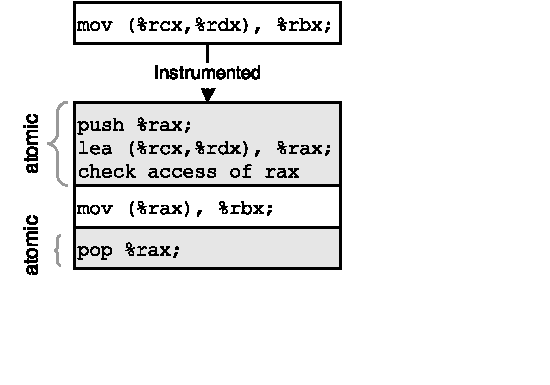
\includegraphics[height=10em,clip=true,trim=0 5em 10em 0]{diagrams/drk_instrumented_mov.pdf}}\vspace{-2.5em}
\columnbreak
\vspace{-1.5em}\hspace{-0.5em}\subfloat[\label{fig:interrupt_delay_granary}Pre and post instrumentation in Granary. The two instrumentation blocks, as well as the native instruction are wrapped in a delay region.]{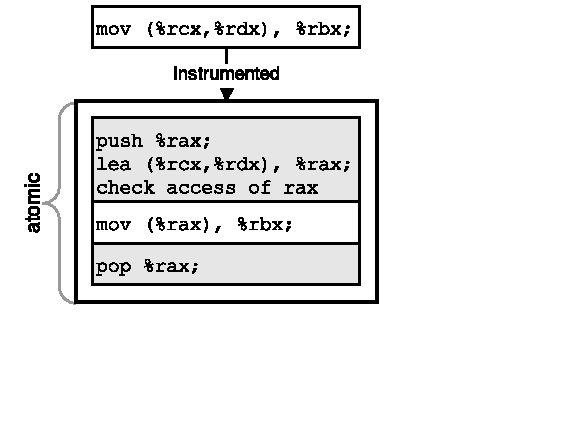
\includegraphics[height=10em,clip=true,trim=0 5em 10em 0]{diagrams/granary_instrumented_mov.pdf}}\vspace{-2.5em}
\end{multicols}
\caption{Example showing equivalent pre- and post-instruction instrumentation with DRK (left) and Granary (right). In DRK, the injected instrumentation instructions (grey) are guaranteed to execute atomically, up until the next native instruction (white). In Granary, no guarantees are made on injected instrumentation, unless otherwise instructed. In this case, a delay region surrounds both the pre- and post-instrumentation, as well as the native instruction, guaranteeing that the entire sequence of instructions execute on the same CPU.}
\end{figure}

One challenge with any DBT system is how it copes with non-reentrant instrumentation. For example, instrumentation that modifies CPU-private data structures cannot be safely executed by a pre-emptive kernel running on an SMP. If the thread being instrumented is interrupted, then the kernel might decide to re-schedule the task to resume its execution on a different CPU. Any modifications to CPU-private state would lead to undefined behavior.

DRK's solution to this problem assumes that all injected instrumentation instructions are potentially non-reentrant, and \emph{delays} interrupts occuring within instrumented code \cite{DRK}. Interrupt delaying allows DRK to maintain the precise interrupt semantics of x86: interrupts and exceptions only arrive on logical instruction boundaries in the native code, and kernel interrupt handlers only observe faults or exceptions at native instruction boundaries. This approach introduces subtle complexity when creating instrumentation that injects instructions both before (pre) and after (post) native instructions.

\Cref{fig:interrupt_delay_drk} shows an example of pre- and post-instrumentation around a \texttt{mov} instruction. If an interrupt arrives within the pre-instrumentation, then DRK delays they delivery of the interrupt until the native instruction (\texttt{mov}). After the interrupt is handled and execution attempts to return to the interrupted instructions, DRK will re-instrument the ``tail" of interrupted basic block, starting from the \texttt{mov} instruction. This involves re-creating the pre- and post-instrumentation of the \texttt{mov} in the tail basic block. When executed, this will result in an unbalanced number of \texttt{push} and \texttt{pop} instructions. That is, \texttt{push \%rax} is executed in both the original and tail basic block, but \texttt{pop \%rax} is only executed in the tail basic block. This is a specific example of a more general problem: DRK's approach to interrupt delaying does not play well with idempotent instrumentation.

%If the pre-instrumentation is not idempotent, then its re-execution will result in undefined behavior. We encountered this issue when using DRK for kernel module instrumentation, where our pre-instrumentation spilled registers to the runtime call stack, and our post-instrumentation restored the spilled registers. Because of interrupt delaying, the spilling code was sometimes repeated many times, whereas the restoring was only executed once. This led to hard-to-debug kernel crashes.

Btkernel provides no solution to the problem of handling non-reentrant instrumentation, beyond requiring that instrumentation tools disable and re-enable interrupts around non-reentrant instrumentation code \cite{btkernel}. Unfortunately, disabling and re-enabling interrupt is costly.

Granary charts a middle ground between the two aforementioned approaches. Most instrumentation is re-entrant, partially because kernel instrumentation tools can depend on the runtime call stack for scratch storage space. However, interrupt delaying is sometimes useful because it enables non-reentrant instrumentation to avoid to continually disable and re-enable interrupts. For example, Granary's basic block tracing tool writes to a CPU-private buffer containing the sequence of executed basic block program counters. Operating on a CPU-private buffer is more efficient than operating on a global buffer because it avoids cache line contention and locking on an SMP. However, writing to a CPU-private buffer is only safe if the entire write executes on the same CPU. An equivalent tool developed for btkernel---which does not support interrupt delaying---would have to disable and the re-enable interrupts around the write. The is inefficient because it introduces flag stalls into the instruction pipeline \cite{AgnerMicroarchitecture}, and because interrupts arrive relatively infrequently.

Granary conveniently solves this problem by allowing instrumentation tools to declare \emph{interrupt delay regions}. An interrupt delay region is a sequence of instructions (which can contain internal control flow) inside of a basic block that must be executed atomically. \Cref{fig:interrupt_delay_granary} shows an interrut delay region that surrounds both the pre- and post-instrumentation of a native \texttt{mov} instruction. If an interrupt arrives anywhere within this region of code, Granary will delay the interrupt to the end of the region. The declarative nature of interrupt delay regions allows instrumentation developers to opt-in to interrupt delaying, and control exactly when, where, and for how long interrupts can be delayed.

Granary implements interrupt delay regions by recording bounds information about interrupt delay regions inside of each basic block's meta-data (\Cref{sec:metadata}). When a basic block is interrupted, Granary inspects the block's meta-data and determines if the interrupt must be delayed. If a delay is required, then all instructions belonging to the delay range are copied into a CPU-private buffer. All instructions are copied because a delay region might contain internal control-flow. A CPU-private buffer is used because the number of CPUs is a natural upper bound on the number of simultaneously executing delay regions. After the copied instructions, Granary emits code that code re-creates the interrupt stack frame, followed by a jump to the interrupt vector (which is controlled by Granary). This jump ensures that Granary's interrupt handler regains control after the instructions within the delay region fully execute, but before the kernel observes the interrupt. When Granary regains control, it can then delegate to the instrumentation tool to handle the interrupt, or defer handling of the interrupt to the kernel.

When all instructions have been emitted to the CPU-private buffer, Granary emulates a return from the interrupt (without issuing an \texttt{iret} instruction). The emulated return leaves interrupts disabled and transfers control to the CPU-private buffer. Leaving interrupts disabled ensures that the remainder of the delay region will execute on the current CPU, and avoids reentrancy issues related to the copied region being located in a CPU-private buffer.

% and re-issues the interrupt to Granary. Granary then emulates a return from the current interrupt handler (without issuing an \texttt{iret} instruction), but leaves interrupts disabled and redirects execution into the copied code.\footnote{Leaving interrupts disabled is required to ensure that executing the copied instructions in the CPU-private buffer is reentrant. Granary performs some sanity checks on the instructions being copied to ensure that they don't re-enable interrupts.} When the copied code finishes, Granary regains control and observes the reconstructed interrupt stack frame. At this point, Granary or the tool can choose to handle the interrupt or defer the handling of the interrupt to the kernel.

%while not supporting delaying has value because not all instrumentation is non-reentrant. By default, Granary does not delay interrupts. However, instrumentation tools can declare \emph{interrupt delay ranges}: 

%, but introduces implementation complexities and high overheads for interrupt-heavy workloads. Precise interrupt delivery is one of the ways which DRK maintains transparency: interrupt handlers only 
%The interaction between DRK's interrupt delaying mechanism and how also makes designing instrumentation subtlely harder. For example, Granary's \toolname{RCUdbg} tool injects instrumentation inside of read-side critical sections that looks for loads/stores from tainted addresses. When necessary, \toolname{RCUdbg} spills and restores registers around each checked load/store operation, so that the registers can be safely used by the checking code. This is an examuple of pre and post instruction instrumentation: some instructions are injected before a native instruction, and some instructions are injected after. DRK is oblivious to the relationship between pre/post instrumentation, and so an interrupt that occurs within the pre-instrumentation will only be delayed until the native instruction.

\subsection{Control Flow Implementation}
\subsubsection{Direct Control Flow}
% Code block showing an example JZ (jump if ZF=1).
\lstset{language=[x64]Assembler}
\newsavebox\nativejcc
\begin{lrbox}{\nativejcc}
\begin{minipage}[b]{4cm}
\begin{lstlisting}[basicstyle=\scriptsize\ttfamily]
cmp $0x0, %rax
jz value_is_zero 
...
( fall through )
\end{lstlisting}
\end{minipage}
\end{lrbox}

\newsavebox\translatedjcc
\begin{lrbox}{\translatedjcc}\begin{minipage}[b]{4cm}\begin{lstlisting}[basicstyle=\scriptsize\ttfamily]
  cmp $0x0, %rax
  jz edge_value_is_zero
  jmp edge_fall_through

edge_value_is_zero:
  call *(jz_patch_data)
edge_fall_through:
  call *(jmp_patch_data)
\end{lstlisting}
\end{minipage}
\end{lrbox}

\begin{figure}[t!]
\subfloat[Native Code]{\usebox\nativejcc}
\hfill
\subfloat[Translated Code]{\usebox\translatedjcc}
\caption{\label{fig:direct_edge_code}Example translation of a conditional control flow instruction (\texttt{jz}) and its edge code. The original \texttt{jz} is translated into a \texttt{jz} that uses a 32-bit relative displacement to transfer control to an edge code function call (\texttt{edge\_value\_is\_zero}). When executed, the function call reads its target from an edge data structure (\texttt{jz\_patch\_data}), which contains all information necessary to resolve the \texttt{jz}'s target and patch the original \texttt{jz}. Patching is performed with a four byte atomic write to the relative displacement operand of the \texttt{jz} instruction. Finally, the return address of the \texttt{call} instruction is altered to transfer control to the newly resolved target.}
\end{figure}
Like btkernel, Granary translates direct control-flow instructions (CTIs) into equivalent jumps into CTI-specific ``edge code" (\Cref{fig:direct_edge_code}). Edge code lives outside the code cache, so as to not pollute the processor's instruction cache \cite{btkernel}.

When control flows through a basic block $B_{pred}$ for the first time, any jumps taken will transfer control to edge code that is specific to the jump taken. Edge code contains only a single indirect \texttt{call} instruction, thus allowing multiple edge codes to occupy a single cache line. The indirect \texttt{call} transfers control to Granary via a function pointer located in an ``edge data structure", which describes how to translate the target basic block, $B_{succ}$. Granary gains control and looks up or translates the target code according instrumentation policy stored in the edge data structure. Then, Granary uses modifies the original CTI in $B_{pred}$ in place so that it transfers control to $B_{succ}$  (\Cref{sec:patching}). Finally, Granary releases control and context switches to $B_{succ}$.

% and is responsible for transferring control from a basic block ($B_{pred}$) to Granary so that the next basic block ($B_{succ}$) can be found/translated, and then connected ($B_{pred} \underset{\texttt{jz}}{\to} B_{succ}$) via hot code patching.

\subsubsection{Indirect Control Flow}\label{sec:ibl}


%Indirect branch lookup through a global, fixed-size hash table. A basic block making an indirect control flow transfer jumps to an in-edge that knows where to find the indirect CTI target (e.g. in a specific register or memory location). The in-edge then uses the target as an index into the hash table, and jumps to the target address stored in the indexed hash table entry. That entry will either be the address of an out-edge, or of Granary's indirect branch resolver. Each out-edge is specific to a target basic block, and first checks if the intended jump target matches the out-edge's target. If so, then control is transfered to the target basic block, otherwise control is transfered either to Granary or to the next out-edge. Granary chains together out-edges through conditional jumps just as 

%Hash table entries are code addresses of out-edge code stub. Each out-edge code stub is specific to a target basic block, and is responsible for checking if the intended control-flow target is the out-edge's target or not. If not, the out-edge either directly jumps to the next out-edge whose target also fits into the same hash table bucket, or jumps to Granary to determine the target basic block.

Granary translates indirect CTIs (\texttt{call}, \texttt{jmp}) into their equivalent direct control flow versions, where the direct versions jump to ``in-edge" code. In-edge code loads the indirect jump target (e.g. a specific register or memory location), saves the flags register, and several scratch registers. Finally, the in-edge uses the indirect target as an index into a global, fixed-size hash table of indirect branch targets. The entries of the hash table either point to Granary or to ``out-edge" code (\Cref{fig:ibl}). 

\begin{figure}[t!]
\vspace{-1.5em}\hspace{4em}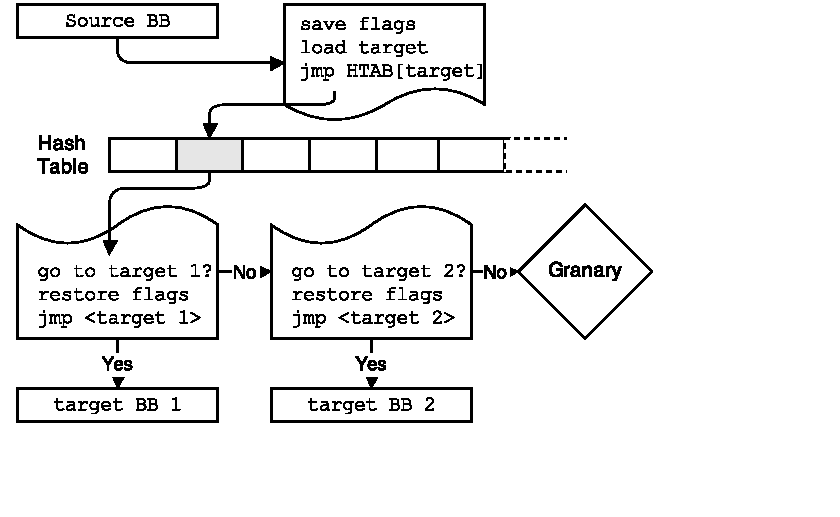
\includegraphics[width=0.9\columnwidth]{diagrams/ibl.pdf}\vspace{-2.5em}
\caption{\label{fig:ibl}Process of resolving an indirect branch. Control transfers from a source basic block, to the in-edge code specific to where the indirect target is stored (e.g. register, memory address), through the global hash table and on to either one or more out-edge code stubs, or to Granary.}
\end{figure}

Out-edge code is specific to a target basic block, and performs the function of separate chaining in the indirect branch lookup hash table. When control transfers to out-edge code, the out-edge checks to see if the indirect target matches the out-edge code's target basic block. If they match, then the out-edge code restores scratch and flags registers and jumps directly to the target basic block. Otherwise, the out-edge code jumps to another out-edge code or to Granary. If one out-edge code block jumps to another one, then the targets of the two out-edge code blocks collide in the global hash table. In this respect, out-edge code is chained together through control flow, just as colliding entries in a typical hash table can be chained together through a linked list.

Granary's use of out-edge code avoids re-entrancy issues related to indirect control flow that present in DRK and btkernel. Both DRK and btkernel store the target of an indirect CTI in a CPU-private memory location. To complete an indirect control transfer, both systems perform (roughly) the following steps: \begin{enumerate}[itemindent=\parindent]%
\setlength{\itemsep}{2pt}%
\setlength{\parskip}{0pt}%
	\item Save the flags and disable interrupts.
	\item Save registers.
	\item Lookup the next basic block address.
	\item Store that address in a CPU private memory location.
	\item Restore registers.
	\item Restore the flags and interrupt state.
	\item Indirectly jump to the target basic block through the CPU-private location.
\end{enumerate} %
However, the ordering of steps (6) and (7) introduce a reentrancy problem: the access to the CPU-private location is not safe because an interrupt might arrive before the indirect jump in step (7). This unusual design is motivated by the constraint that the entire lookup procedure must save (2) and restore (5) the register state for correctness, but must also save the target pc \emph{somewhere} so that execution can eventually be redirected. Granary's out-edge code avoids this reentrancy issue by having the out edge code itself (in the form of a direct \texttt{jmp}) contain the target pc.

%If an entry points to Granary, then no as-of-yet resolved indirect jump target hashes to that entry.

%Granary implements separate chaining through code (i.e. control flow jumps, as opposed to date, e.g. linked list pointers)
%In the event that one-or-more indirect jump targets do hash to an existing entry
%In-edge code is responsible for 
% to first search for their targets in a global, fixed-size hash table, and failing that, context-switch into Granary to perform a full lookup and potential translation.
%using a fixed-size hash table, where the native target of the indirect 

\subsection{Optimizations}

\subsubsection{Ahead-of-time Translation} \label{sec:aot}
Granary ends basic blocks at conditional branches (\texttt{jCC}), direct and indirect \texttt{jmp}s, and \texttt{ret}s and \texttt{iret}s. Basic blocks ending in conditional branches are extended to contain two trailing CTIs: a copy of the native \texttt{jCC}, and a synthesized direct \texttt{jmp} to the code executed when the condition code is not set (i.e. when the conditional jump is not taken).

If a basic block ends in either a copy of a native direct \texttt{jmp} or synthesized direct \texttt{jmp}, then Granary will perform ahead-of-time translation and instrumentation of the targeted basic block. The repeated application of translating \texttt{jmp} targets forms traces in Granary's code cache. Granary optimizes traces by directly connecting basic blocks together when there is internal control flow within the blocks of the trace, and by eliding synthesized \texttt{jmp}s between adjacent basic blocks.

Granary's tracing strategy is based on the observation that the most commonly executed path through code follows a straight line. That is, execution is more likely to fall through a conditional CTI than it is to take the conditional CTI. We experimentally verified Granary's tracing strategy by disabling tracing and relying on Granary's performance counters to count how many conditional branches were patched (by their edge code), versus how many synthesized fall-through \texttt{jmp}s were patched.

%using internal performance counters within Granary

%Static branch prediction hints (\texttt{likely}, \texttt{unlikely} macros) are heavily used in the Linux kernel source code. Although static branch prediction hints can be specified on individual conditional branch instructions, recent x86-based architectures ignore these hints \cite{AgnerMicroarchitecture}. Therefore, static branch prediction hints at the source code level mainly affect compiler optimizations, including intraprocedural basic block scheduling. Our tracing strategy is based on 

%Tr

%We expect and have experimentally verified that the most common execution path through code is straight-line and does not following conditional branches.

%Due to instruction prefetching, we expect that the likely or

%On recent x86-based architectures, these hints only affect the schedule of basic blocks in the intraprocedural control-flow graph \cite{AgnerMicroarchitecture}.

\subsubsection{Patching and Alignment}\label{sec:patching}
For efficiency, basic blocks in Granary's code cache are directly connected through direct control flow instructions (\texttt{call}, \texttt{jmp}, \texttt{jCC}). That is, if there is a direct branch from one native instruction to another, then there will be a corresponding direct branch between two translated instructions in Granary's code cache.

Granary opportunistically connects two basic blocks together using a direct branch if \begin{inparaenum}[i)]
	\item the branch transfers control to another basic block within the current trace; or
	\item the branch transfers control to an already translated basic block.
\end{inparaenum} However, not all basic blocks can be connected at translation time, therefore Granary employs edge code and hot-code patching (\Cref{fig:direct_edge_code}) to connect basic blocks at runtime.

Granary atomically patches direct CTIs that target edge code to instead point to their (now resolved) target basic block. Due to limitations of the x86 architecture, atomic operations cannot straddle cache lines. Therefore, patchable instructions (or parts thereof) must be aligned so as to not straddle two cache lines.

%Padding basic blocks so as to align specific instructions must not change the execution behavior. 

One approach to change an instruction's alignment is to pad the basic block with additional \texttt{nop} instructions. An alternative when more than a few bytes of padding are needed is to introduce a single control-flow instruction (\texttt{jmp}) that jumps around the padded area. However, adding extra instructions introduces latency into the fetch/decode/execute cycle. Therefore, when possible, Granary uses ignored instruction prefixes to alter an instruction's alignment. For example, Granary aligns patchable conditional jumps using static branch prediction hint prefixes, which are ignored by recent x86 processors \cite{AgnerMicroarchitecture}. Finally, most basic blocks are small (i.e. fit in one cache line), therefore, aligning basic blocks on a cache line boundary naturally avoids the potential for a patchable instruction to straddle two cache lines.

%To reduce the overhead of alignment 
%In some cases, basic blocks can be directly connected during basic block translation time. For example, intra-trace CTIs, or CTIs targeting already translated basic blocks. However, not all basic blocks can be connected this way, therefore some runtime 
%Granary connects some basic blocks at translation time (e.g. intra-trace control-flow instructions). This is common when tracing is enabled, but also occurs when a branch targets an already translated basic block. However, 
%Some basic blocks are directly connected at basic block translation time. One example is branches that target other basic blocks within a trace. Another example is a branch to an already translated basic block.
%Other basic blocks are only connected at runtime. For example, if the function \texttt{memset} has never been executed, then a \texttt{call} to \texttt{memset} will be translated to target edge code (\Cref{fig:direct_edge_code}) that, when executed, will translate \texttt{memset}'s first basic block and patch the \texttt{call} to target the translated basic block.
%For example, the targets of function call instruction (\texttt{call}) are resolved just-in-time (unless the target is already known). For each translated \texttt{call} instruction, Granary generates edge code (\Cref{fig:direct_edge_code}) that will find or translate the first basic block of the function being called, and patch the translated \texttt{call} instruction to point to the function's first basic block.
%For example, if a direct branch in one basic block targets another block within the trace under construction, then that 
%Basic blocks are directly connected at block translation time when branches in traces re-enter a trace, or when branches target previously translated basic blocks. If a branch does not target another basic block within its trace, or does not target a previously translated basic block, then the branch will target edge code that will resolve that branches target at runtime.
% However, when a given basic block is translated, not all of its targets are known (e.g. \texttt{call} and \texttt{jCC} targets). Therefore, edge code (\Cref{fig:direct_edge_code}) is generated that translates/resolves a branch target when that branch is first executed, and patches the translated branch to avoi
% The targets of some of these direct CTIs are only resolved at runtime, by executing edge code. As an optimization, jumps to edge code are dynamically patched to transfer control to their intended targeted basic blocks.
%edge code use hot code patching to update a translated CTI to redirect execution 

\subsubsection{Trace Allocation}\label{sec:trace_alloc}
Arranging for commonly executed sequences of basic blocks to appear adjacent in memory, also called tracing, typically improves the runtime performance of instrumented programs \cite{DynamoRIO}. Typical approaches to tracing require a runtime profiling infrastructure (e.g. recording basic block execution counts). Granary attempts to reap the benefits of tracing without the runtime profiling overhead by opportunistically forming traces using ahead-of-time translation (\Cref{sec:aot}), and by arranging for related basic blocks to be allocated sequentially in memory.

Two basic blocks $B_1$ and $B_2$ are ``related" ($B_1 \to B_2$) if there is a control flow instruction from $B_1$ to $B_2$. Granary arranges for $B_2$ to be allocated nearby or adjacent to $B_1$ by allocating $B_2$'s instructions from the same pool of memory used to allocate $B_1$'s instructions. The base case of this induction are kernel entrypoints. For example, each system call is an entrypoint into the kernel, and is associated with a private memory pool. When a system call is executed for the first time, the basic blocks needed to fulfill the system call's computation are allocated from that system call's memory pool.

To avoid translation conflicts (e.g. on utility functions being simultaneously executed by distinct system calls), and to improve the predictability and reproducability of a given code cache layout, Granary can delay the takeover of kernel entrypoints. That is, Granary can take over one entrypoint at a time, and wait for a specified period of time before taking over the next entrypoint. The effect of delaying the takeover process is that it increases the chances that a given entrypoint (e.g. a blocking system call) will execute to completion, and thus have all of its basic blocks  arranged sequentially in memory.

Trace allocation is implemented by recording the memory pool used to allocate a given basic block in that basic block's meta-data. When Granary needs to translate a new basic block, it inspects the predecessor basic block's meta-data and uses the predecessor basic block's memory pool to service allocation requests for the basic block in translation.

%, and is associated with a private memory pool from which to allocate memory for basic blocks. The net result is that most of the basic blocks eecuted in service of a single system call are allocated from that system call's memory pool.
%The intuition for this approach is that kernel code is not very ``loopy", and so 
%Granary services memory allocation requests for basic block instructions from memory pools. By default, Granary has as many memory pools as there are CPUs. However, when trace allocation is enabled
%Tracing is also beneficial for 
%However, tracing of this sort requires mechnisms for evicting stale basic blocks, 
%Constructing traces of ``hot'' 
%JIT generally results in better performance .
%By default, Granary allocates the memory needed to hold the instructions of a basic block from CPU-private memory pools. Each memory pool serves basic block allocation requests out of fixed-size memory blocks, ranging from 4K to 24K in size.

\subsubsection{System Calls}

Granary treats indirect \texttt{jmp}s or \texttt{call}s through the Linux kernel system call table specially. The Linux kernel (as of Linux 3.12) has approximately 300 distinct system call targets, some of which are executed often. To avoid polluting the indirect branch lookup hash table with these targets (\Cref{sec:ibl}), and to avoid the indirect branch lookup overhead, Granary creates a separate, \emph{shadow} system call table.

%re-direct jumps through the system call table 

Granary's translation post-processing mechanism identifies indirect control flow through the system call table and alters those CTIs to direct control flow through the shadow system call table instead. The entries of the shadow system call table are ``lazy" entrypoint translator functions. Upon their first execution, these entrypoint translators find or translate the first basic block of the system call handler, and update the shadow system call table accordingly. 

%Directing control through the shadow system call table avoids the overhead of going through the indirect branch lookup (IBL) table (\Cref{sec:ibl}), and reduces the number of potential conflicts in the IBL table.
% whose entries are code cache basic block addresses translated according to the starting instrumentation policy.
%\subsection{Reproducability}
%Hello

\section{Specializing on What to Instrument}\label{sec:what}

\begin{figure}
\captionsetup[subfloat]{width=0.45\columnwidth}
\begin{tabularx}{\columnwidth}{XX}%
\subfloat[Full kernel instrumentation.]{\hspace{2.5em}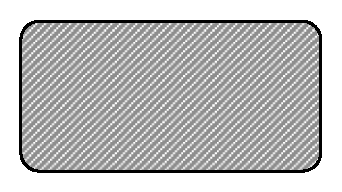
\epsfig{file=diagrams/kernel.eps,width=0.125\textwidth}} & %
\subfloat[Module-only instrumentation]{\hspace{2.5em}
\epsfig{file=diagrams/module.eps,width=0.125\textwidth}} \\
\subfloat[Module-only instrumentation, with a function specialized to run natively by using a module function wrapper.]{\hspace{2.5em}
\epsfig{file=diagrams/module_wrapper.eps,width=0.125\textwidth}} & %
\subfloat[\label{fig:module_probe}Module-only instrumentation, with a kernel function specialized to also be instrumented by using a probe-based wrapper.]{\hspace{2.5em}
\epsfig{file=diagrams/module_probe.eps,width=0.125\textwidth}}
\end{tabularx}
\caption{Example of using different granularities of instrumentation to selectively instrument or not instrument specific code.}
\end{figure}

\begin{figure*}[ht!]
\lstset{language=C, tabsize=2, stepnumber=1}
\begin{multicols}{2}
\begin{lstlisting}[basicstyle=\scriptsize\ttfamily]
struct device_driver {
  ...
  int  (*probe)(struct device *);
  int  (*remove)(struct device *);
  void (*shutdown)(struct device *);
  int  (*suspend)(struct device *, pm_message_t);
  int  (*resume)(struct device *);
  ...
  const struct dev_pm_ops *pm;
  ...
};
\end{lstlisting}
\columnbreak
\begin{lstlisting}[basicstyle=\scriptsize\ttfamily]
TYPE_WRAPPER(struct device_driver, {
  PRE_OUT {
    ABORT_IF_FUNCTION_IS_WRAPPED(arg.probe)
    WRAP_FUNCTION(arg.probe);
    WRAP_FUNCTION(arg.remove);
    ...
  }
  POST_OUT {
    POST_WRAP(arg.pm);
  }
})
\end{lstlisting}
\end{multicols}
\caption{The Linux device driver structure is shown on the left. The automatically generated type wrapper for this structure is shown on the right. In the wrapper code, \texttt{arg} is a reference to a \texttt{struct device\_driver} object passed as, or referenced by, an argument to a kernel or module wrapper. Code in the \texttt{PRE\_OUT} section is applied to arguments of the wrapped type before a kernel wrapper is invoked. Similarly, code in the \texttt{POST\_OUT} section is applied to arguments of the wrapped type after a kernel wrapper is invoked. \texttt{POST\_WRAP} invokes the type wrapper that is specific to the value to which it is applied (\texttt{arg.pm}). Type wrappers also support \texttt{\_IN} suffixes instead of \texttt{\_OUT} suffixes, which apply to data going into modules (i.e., over module wrappers). Finally, the \texttt{RETURN\_} prefix is used to apply some code to return values of either kernel or module wrappers.}
\label{fig:type_wrapper}
\end{figure*}

Granary allows tool developers to precisely specify what code should be instrumented. Example granularities of instrumentation include the whole kernel, only specific modules, only specific functions, or on-demand instrumentation based on events (e.g. interrupts or exceptions).

\subsection{Kernel}
Like DRK and btkernel, Granary can instrument the whole kernel. Instrumenting the whole kernel requires interposing on the system call entrypoint (x86-64 \texttt{MSR\_LSTAR} model-specific register) and on the interrupt vector entrypoints (stored in the interrupt descriptor table). For whole-kernel instrumentation, Granary boostraps by duplicating the the early entrypoint instructions that are responsible for switching execution onto a kernel stack, and then injects a jump to translate/instrumented kernel code after the stack switch. The translation process continues when a system call or interrupt occurs and follows the jump from duplicated into translated code. Granary only translate code that is known to operate on a kernel stack so that instrumentation tools can safely save transient data in a reentrant way by spilling that data to the stack.

\subsection{Modules}\label{sec:module}

Unlike DRK and btkernel, Granary can target instrumentation only at specific kernel modules, while executing the rest of the kernel natively and without overhead. Instrumenting only specific kernel modules is particularly useful for debugging tools because modules represent the bulk of new kernel code under development, and contain the most bugs \cite{FaultsInLinux}.

Granary interposes on an existing module by using hardware page protection to mark an existing module as non-executable and trap attempts to execute that module's code. Granary transparently recovers from these traps by returning execution to instrumented code. Granary takes control of dynamically loaded modules by interposing on the Linux kernel's module loading process. When a kernel module is loaded, Granary bootstraps by translating the first basic block of the module's initialization function.  It then replaces the pointer to that function with a pointer to the translated basic block. The translation process continues when the kernel initializes the module by invoking the translated module code. As with existing modules, the native code segments of dynamically loaded modules are page protected to prevent and recover from accidental execution. 

While correct, hardware page protection is an inefficient mechanism for gaining control of module code execution. That is, after the (instrumented) module initializer runs to completion, Granary needs an efficient way to regain control of future invocations of the module's code. Our approach to regaining control is based on the observation that modules tell the kernel about their interfaces by registering functions with the kernel. We expect that at least some of the registered functions will be executed by the kernel because this is the mechanism by which modules extend the kernel's functionality. To Granary, registered module functions represent potential future \emph{attach} points, where a switch from native to instrumented execution will occur. Furthermore, Granary discovers additional attach points at detach points by observing pointers to module functions that are passed by modules to the kernel.

Granary uses static analysis to dynamically discover attach points by wrapping the kernel/module interface. Kernel functions are wrapped by \emph{kernel wrappers} that inspect and traverse argument pointers in search of pointers to module functions. \Cref{fig:type_wrapper} shows an example of a type wrapper for the Linux device driver structure. If a pointer to a module function (a future attach point) is discovered, then Granary replaces that pointer with a function-specific \emph{module wrapper}. Granary inspects and modifies arguments to module wrappers in the same way as for kernel wrappers. This allows Granary to discover kernel entry points that will cause instrumentation to detach. Finally, Granary redirects execution to the appropriate kernel or instrumented module function after wrapping has occurred.

Kernel and module wrappers invoke \emph{type wrappers} to find and wrap pointers to module functions that are directly or indirectly referenced by kernel/module function arguments. A type wrapper is a function that recursively  traverses the in-memory object graph and converts pointers to module code into pointers to wrapped module functions. Type and kernel wrappers are automatically generated at Granary's compile time by scripts that statically analyze the kernel source code. Granary automatically matches any variable in a kernel wrapper to a type wrapper if the base type (absent pointers, specifiers, and qualifiers) of that variable matches the type wrapper's wrapped type. Similarly, Granary automatically generates module wrappers using a combination of compile-time meta-programming and runtime code generation to match type wrappers to the declared arguments of \texttt{C} function pointer types.  Granary's wrapper approach has two benefits: (i) it is more efficient than the trap-based alternative, and (ii) it gives instrumentation tools direct and semantically meaningful access to data crossing the kernel/module boundary.

\label{sec:implicit_attach}
After Granary bootstraps on the module initialization process, \emph{attaching} occurs in one of three ways: \begin{enumerate}
	\item {\bf Implicit attaching:} the kernel returns to instrumented module code in the code cache. This occurs when instrumented moduel code is interrupted, or when the module invokes a kernel function (detaching) and that function returns to the instrumented module code (attaching).
	\item {\bf Fast attaching:} the kernel invokes a wrapped module function. The first instance of fast attaching for any kernel module is when the kernel's module loader invokes the instrumented module initializer function. 
	\item {\bf Slow attaching:} the kernel invokes unwrapped module code. If the kernel executes a module function which was passed to the kernel in a type-unsafe manner, then the processor will raise a fault because Granary uses hardware page protection to prevent module code from being executed. Granary handles these faults by returning execution to the instrumented version of the faulting module code.
\end{enumerate}

\label{sec:detach}
Granary \emph{detaches} when control transfers from instrumented code to native (uninstrumented) code. Detaching occurs in one of two ways: \begin{enumerate}
	\item {\bf Implicit detaching:} instrumented module code returns to the kernel code which originally invoked the module, or is interrupted (initial interrupt handling is done by the kernel).
	\item {\bf Wrapped detaching:} instrumented module code invokes a kernel wrapper, which later transfers control to the kernel.
\end{enumerate}

Granary's wrappers expose a wealth of static program information to instrumentation tools. Instrumentation tools can use information present in wrappers to alter how code is instrumented, or to simply inspect the runtime object graph in a type-safe way. For example, we are actively using type information present in wrappers to create a tool that generates models of typical module behavior. The wrapper information serves two roles in our tool. First, we use type wrappers to assign type-specific IDs to module-allocated memory that is shared across the module/kernel interface. Type ID assignment is critical because it allows us to match memory reads and writes to specific kernel data structure fields. Second, we use the kernel and module function wrappers to generate call graphs of a module's execution. This call graph models module behavior (according to the kernel) because we label module code nodes with kernel data structure and function pointer field names (derived from module wrappers). This labelling allows us to generalize across similar modules. For example, code reached by calling the \texttt{ext4\_mount} and \texttt{btrfs\_mount} functions from the \texttt{ext4} and \texttt{btrfs} file system modules, respectively, are both labelled as \texttt{file\_system\_type::mount}, because the function addresses are stored (and later replaced by module wrappers) in the \texttt{mount} field of a \texttt{file\_system\_type} data structure. The combined records from multiple ``trusted'' modules of the same class (e.g., mature, open-source file systems) models the behavior of typical kernel modules. We hope that these models will help us build tools that classify and identify spurious module behavior. 

\subsection{Functions}\label{sec:function_wrapper}

Granary can instrument or not instrument functions in several different ways. For example, \emph{probe-based} instrumentation allows Granary to selectively instrument only a particular function, while \emph{wrapper-based} instrumentation allows Granary to isolate a particular function that is invoked by instrumented code, and choose to instrument that function or run it natively (all while having the flexibility to arbitrarily inspect that function's arguments and return values in a type-safe way).

\subsubsection{Probe-based instrumentation}

Probe-based instrumentation allows an instrumentation tool to replace \emph{all} executions of a particular kernel function, regardless of whether or not the replaced function is executed by native or instrumented code \cite{KProbes, AnyWhereAnyTimeDBT, KernInst}. Probe-based instrumentation can be used to wrap a particular function without instrumenting its code, or to wrap and instrument the probed function's code.

Probe-based instrumentation provides visibility into specific kernel events (e.g. memory allocations) to instrumentation tools that don't instrument the whole kernel (e.g. module-only, \Cref{fig:module_probe}). One example tool that combines module-only and probe-based instrumentation is Granary's kernel module memory leak detector. This leak detector finds leaks of module-owned memory. We say that the some memory is owned by a module iff that memory is deallocated by a module. Unfortunately, ownership of module-allocated memory (for an arbitrary, binary module) is not known \emph{a priori}. Therefore, our tool conservatively assumes that all module-allocated memory is module-owned, unless it is freed by the kernel (observed via probe-based instrumentation of a kernel memory deallocator). We also use probe-based instrumentation to assign module ownership to kernel-allocated \texttt{sk\_buff} data structures, which are allocated by the kernel but deallocated by network device driver modules.

\subsubsection{Wrapper-based instrumentation}

Wrapper-based instrumentation makes use of the same wrapper capabilities used by module-only instrumentation (\Cref{sec:module}), but is available regardless of the instrumentation granularity. Wrapper-based instrumentation is similar to probe-based instrumentation, but permits more selectivity in terms of the context in which the function will be wrapped. That is, a function can be wrapped in one way when executed by instrumented kernel code, and in another way when executed by instrumented module code. Finer-grained selectivity can be achieved by having individual instrumentation policies manually decide how to wrap a given function.

\begin{figure}[t!]
\lstset{language=C, tabsize=2, stepnumber=1}
\begin{lstlisting}[basicstyle=\scriptsize\ttfamily]
MODULE_FUNCTION_WRAPPER(__kmalloc, (size, gfp), {
  void *addr = __kmalloc(size, gfp);
  if(is_valid_address(addr)) {
    add_watchpoint(addr, addr, size);
  }
  return addr;
})
\end{lstlisting}
\caption{Example module function wrapper for the \texttt{\_\_kmalloc} function. This wrapper adds an ``address watchpoint" to the address returned by the kernel's \texttt{\_\_kmalloc} memory allocator. Granary's module memory leak detector uses address watchpoints to track the liveness of module-allocated memory. Every access of a ``watched address" marks the associated memory as live within the current epoch. Memory that has not been live for several consecutive epochs is treated as a potential leak, and a is checked for reachability using a heap memory scanner.}
\label{fig:malloc_wrapper}
\end{figure}

Granary's module memory leak detector is one example application that uses the selectivity of wrappers (with respect to their calling context) to distinguish between module-allocated and kernel-allocated memory. \Cref{fig:malloc_wrapper} shows a module function wrapper that adds ``address watchpoints"  \cite{BehaveOrBeWatched} to module-allocated memory.

%Granary can instrument, or not instrument, particular function

\subsection{On-demand}

On-demand instrumentation makes use of Granary's control over interrupt and exception handling. When a specific exception or interrupt occurs, a Granary tool can turn on instrumentation for the interrupted code. This ties in well with Granary's address watchpoints system, which taints memory addresses by changing their high-order 16 bits into a ``non-canonical" form. Watched addresses trap when accessed by native code, which introduces an opportunity for on-demand instrumentation to be enabled. Another application of on-demand instrumentation is data watchpoints based on hardware page protection and memory shadowing.

Turning on instrumentation when specific data is accessed makes on-demand instrumentation inherently \emph{data-centric} as opposed to \emph{code-centric}. That is, instrumentation is targeted at instructions accessing specific data, instead of the typical ``dragnet" approach employed by most DBT systems, which instrument all memory loads/stores so as to capture the select few that access key data.

% instrumentation turns on when specific data is accessed, and can be turned off at the granularity of an instruction, a basic block, the current executing function, or the current executing task/thread. 

%\section{Mixed-Mode Execution}\label{sec:modes}
%Granary supports two modes of execution: instrumented and native. Module code is instrumented and executes from Granary's code cache, which is under Granary's control. Non-module kernel code runs natively. A mode switch occurs when execution transfers between native and instrumented code. Some mode switches happen naturally (e.g., when instrumented code returns to native code) and other mode switches are mediated by Granary (e.g., when instrumented module code invokes a kernel function).
%
%The mode switch from instrumented module code to native kernel code is easier to detect since the instrumented code runs under Granary's control. Granary treats all kernel functions as \emph{detach} points, where a mode switch from instrumented to native code occurs. At these points, Granary stops executing.
%
%However, Granary needs a way to regain control when native kernel code invokes module code. Our fallback solution for regaining control uses hardware page protection to trap attempts by the kernel to execute native module code. We handle these traps by redirecting execution to instrumented module code. While comprehensive, this approach is not ideal because: \begin{inparaenum}[i)]
%	\item trapping on every execution attempt introduces overhead; and
%	\item the trap does not provide sufficient information about which interfaces were being used by the kernel to invoke the module.
%\end{inparaenum}


\section{Specializing on How to Instrument}\label{sec:how}

Granary gives tools the ability to be selective about what is instrumented. A natural extension of this selectivity is to allow tools to specialize how code is instrumented by dynamically switching the policy used to instrument code. Specialization is desirable in several cases. For example, some instrumentation is high-overhead, but does not need to be applied to all code. One example of this is Granary's \toolname{RCUdbg} tool, which instruments read-side and write-side critical sections more heavily than the rest of code. Unfortunately, existing DBT systems fall short in their support for runtime code specialization \cite{DRK,btkernel,Pin,DynamoRIO}. 

To implement the equivalent of \toolname{RCUdbg}'s runtime code specialization using an existing DBT system requires that a tool developer maintain, update, and check runtime state to know whether or not code is executing inside or outside of a read-side critical section. If a basic block is executing in a read-side critical section, then instrumentation should be enabled, and if it's not in a read-side critical section then it should be disabled. Enabling/disabling instrumentation might be done at the instruction granularity, which introduces at least one branch instruction per native instruction, or at the granularity of basic blocks, which requires generating two copies of each native basic block, where a single branch at the beginning of a basic block chooses between the instrumented or uninstrumented version. Up until now, it has been assumed that there is a mechanism for maintaing state that consistently tracks the current execution context of kernel code (inside vs. outside of a read-side critical section). However, maintaining state in a way that is reentrant and resilient again arbitrary pre-emption and resumption is onerous.

%Existing systems move the burden of code specialization to instrumentation tool developers. 

Fortunately for tool developers, Granary has built-in support for runtime code specialization that does not require manual state management or cause code cache bloat. Granary approach to runtime code specialization uses a technique called \emph{context-driven instrumentation}.

%For example, instrumenting only module code allows Granary to specialize the execution of native code. In the same way, policy switching allows Granary's \toolname{RCUdbg} tool to specialize the execution of instrumented code executing inside of read-side and write-side critical sections. In fact, optimizing the performance of an early Granary tool was the original motivation for policy switching.

\subsection{Context-Driven Instrumentation}\label{sec:policies}

%We developed a Granary tool that detects several Read-Copy-Update (RCU) API misuses in module code. Our tool focused on read-side critical sections (delimited by calls to \texttt{rcu\_read\_lock} and \texttt{rcu\_read\_unlock} in the code), however, most code executes outside of read-side critical sections. As an optimization, we wanted our heavyweight API-checking instrumentation to apply only when the code was executing within a read-side critical section. Implementing this optimization was challenging because each basic block was only translated once, and we had no way to know whether or not the heavyweight instrumentation should be applied to it. Knowing the state (within or outside a read-side critical section) at translation time was not sufficient, since the same translated block could later be executed in the opposite context. That is, code executing \emph{within} a read-side critical section may have originally been translated while executing \emph{outside} of a read-side critical section, and would thus omit the heavyweight API-checking instrumentation. This omission could cause our tool to miss bugs (i.e., it would not be comprehensive) when the basic block executes within a read-side critical section.

%To implement this optimization, 

Granary enables specializing instrumentation to the context in which the instrumented code will execute. Specialization is achieved by allowing multiple, differently instrumented versions of the same code to co-exist within Granary's code cache. That is, if the next basic block to execute has not yet been translated/instrumented for the current execution context, then a new version of that basic block will be created  specifically for the the current execution context.



%In the case of our \toolname{RCUdbg}, there were three execution contexts: within and outside of a read-side critical section. If the same module basic block is  executed in the two contexts, then Granary's code cache would contain two different instrumented versions of that basic block. The way that Granary distinguishes between different execution contexts is with \emph{instrumentation policies}. 

Granary tools identify execution contexts by creating instrumentation policies. An instrumentation policy is both a name for an execution context, as well as a function that decides how to instrument basic blocks that will execute within that context. All tools define an initial policy that Granary uses to instrument module code. Tools are not limited to one policy though: any policy can declare a policy switch that will take effect when a selected control-transferring instruction (CTI) is executed. The effect of a tool specifying a policy switch on a CTI is that the basic block(s) targeted by that CTI will be instrumented according to the specified policy. CTIs with unspecified policies inherit their policies from their containing basic blocks.

For example, our \toolname{RCUdbg} invokes a policy switch from policy $P_{\mathit{null}}$ to policy $P_{\mathit{read\_critical}}$ when $P_{\mathit{null}}$'s instrumentation function observes a \texttt{call} instruction to the \texttt{rcu\_read\_lock} Linux kernel function. A similar switch occurs from $P_{\mathit{read\_critical}}$ back to $P_{\mathit{null}}$ at a \texttt{rcu\_read\_unlock}. Specialization that distinguishes between the inside and outside of read-side critical sections allows \toolname{RCUdbg} to do heavy-weight checks on functions like \texttt{memset}, but only when \texttt{memset} is invoked from within a read-side critical section.

Because policies name an execution context, they also represent states in a finite state machine. That is, code cache execution is in the state named by a policy if the  executing code was instrumented by that policy. A state transition occurs when control transfers from code instrumented by one policy to code instrumented by another policy. A limitation with this approach is that a single state does not encode the sequence of previous states that led to execution being in the current state. For example, RCU permits nested read-side critical sections. If two read-side critical sections are nested then switching from $P_{\mathit{read\_critical}}$ to $P_{\mathit{null}}$ on the first \texttt{call} to \texttt{rcu\_read\_unlock} meant that our tool would lose track of being in the context of the outer read-side critical section.  \toolname{RCUdbg} solves this problem by tracking the nesting depth of RCU read-side critical sections using policies, e.g. $P_{\mathit{read\_critical}_1}$, $P_{\mathit{read\_critical}_2}$, etc.

An alternative and sometimes more powerful model for policy switching is to prevent policy switching on function return instructions (e.g. either through manually specifying a policy switch, or by inheriting the policy from the basic block containing the \texttt{ret} instruction). In most cases, function returns are natural policy reverting points. This is because the current instruction pointer (program counter) encodes the current execution context (by being in a basic block instrumented by some policy), and the code cache return addresses stored on the runtime call stack encode all previous execution contexts. This asymmetry between \texttt{call}s and \texttt{ret}s yields a more powerful context-tracking state machine: \texttt{call}s place contextual breadcrumbs (in the form of return addresses) on the runtime call stack, and \texttt{ret}s read these breadcrumbs to return to a previous context. Policy switches under this lens behave similarly to state transitions in a pushdown automaton; \texttt{call} instructions push a new state onto the stack for each function, \texttt{ret} instructions pop the current function's state from the stack, and other CTIs induce state transitions within the current function by altering control flow.

Granary implements policy tracking and switching by encoding policy information into the meta-data and CTIs of basic blocks. \Cref{fig:direct_edge_code} shows an example of how policy information is directly recorded into control-transfer edge code. If a policy switch is not specified on an instrumented CTI then that CTI inherits the policy used to instrument the basic block containing the CTI. When an instrumented CTI executes for the first time, it yields control to Granary with the CTI target and policy information as inputs. Granary decodes and instruments the targeted instructions according to the input policy information. Because Granary's translation mechanism depends only on CTI policy and target information, Granary is able to ensure that policy information is never lost or corrupted, even in the face of concurrent executions of the same module code, arbitrary pre-emption, and arbitrary resumption.


\section{Application: Control-Flow Graphs}\label{sec:cfg}

\section{Application: RCUdbg}\label{sec:rcudbg}

Read-Copy-Update (RCU) is a scalable, lock-free synchronization mechanism used in the Linux kernel \cite{RCU,RCUInLinux}. When correctly used, RCU permits concurrent reads and writes to shared data structures, but requires that writers synchronize among themselves. Like other synchronization mechanisms, RCU has a deceptively simple API. Misuses of the API can result in hard-to-find bugs that can be implementation-specific (i.e. bugs that manifest in one version of RCU but not another) or architecture-specific (e.g. bugs that only exhibit on architectures with a relaxed memory model). For example, RCU bugs sometimes manifest as use-after-free bugs, which can result in silent data corruption (if the underlying memory remains used) or kernel panics. 



% (assuming that pointer reachability is sufficient to determine semantic reachability in this case).

Granary's \toolname{RCUdbg} tool is designed to catch RCU bugs related to kernel code misusing pointers to RCU-protected data structures. The following is a non-exhaustive list of requirements that must be met by reader and writer threads operating on an RCU-protected data structure. The list omits a description of how RCU-protected data structures are garbage collected, which is beyond the scope of the bugs caught by \toolname{RCUdbg}.

%the associated memory may or may not be free, but the data structure occupying that memory can't be proven to exist. This 

%  However, this class of RCU bugs is not well-suited to being detected by a use-after-free memory checker tool
%RCU is notoriously hard to use, despite its relatively simple API. RCU usage bugs, like bugs with other synchronization mechanisms, often stay hidden and only exhibit themselves for very specific thread interleavings/schedules.



% go silently unnoticed because the memory 


%While bugs related to mutual exlusion locks might result in easily observable deadlocks, bugs related to RCU typically result in use-after-free errors, which sometimes go silently unnoticed, sometimes result in kernel panics, and most of the time work as expected because the associated data is .

\begin{enumerate}
	\item Readers must tolerate an inconsistent view of the shared data structure. That is, a reader operating concurrently with a writer might observe either the version of the data before or after the writer's changes have been published. This can be complicated when writers perform multiple, discrete updates to a data structure. One example of this is a doubly linked list: a writer that is adding a new entry into a doubly linked list must update at least two RCU-protected pointers.
	
	\item Readers must operate within \emph{read-side} critical sections, which are delimited by \texttt{rcu\_read\_lock} and \texttt{rcu\_read\_unlock}, respectively.
	
	\item Within read-side critical sections, readers can only read a shared data structure after obtaining a pointer to that shared data structure using the \texttt{rcu\_dereference} API function. An RCU-protected pointer is like a normal pointer, but points to a potentially incomplete or partially-constructed data structure. \texttt{rcu\_dereference} operates on an RCU-protected pointer and returns an ``unprotected" version of the pointer. The reader can use the unprotected pointer to safely access the shared data structure within the remainder of the its read-side critical section. If \texttt{rcu\_dereference} is not used, then the reader might observe a partially-constructed (i.e. incomplete) version of the shared data structure. Notably, accessing the original data structure and not the dereferenced data structure pointer--even after an \texttt{rcu\_dereference}--is undefined behavior. That is, within a read-side critical section, RCU only guarantees the ``completeness" of data structures pointed to by RCU-dereferenced pointers. Data accessed within a read-side critical section is \emph{not} guaranteed to exist outside the read-side critical section.

	\item Writers must synchronize among themselves before any writes to a shared data structure are performed. Synchronization is typically achieved via mutual exclusion locks, spin locks, or by having a single, designated writer thread. We say writes to the shared data structure occur within \emph{write-side} critical sections.

	\item RCU only defines how writers can update RCU-protected pointer within a shared data structure. Modification of non-RCU-protected pointer fields within an RCU-protected data structure is beyond the scope of RCU's correctness guarantees.

	\item Writers wishing to update an RCU-protected pointer in a shared data structure must use the \texttt{rcu\_assign\_pointer} API function. \texttt{rcu\_assign\_pointer} assigns a new value to an RCU-protected pointer in a shared data structure.

	\item Readers must access any pointer field operated on by an \texttt{rcu\_\linebreak[0]assign\_pointer} using \texttt{rcu\_\linebreak[0]dereference}. For example, if the \texttt{next} pointer field in \emph{any} list element of an RCU-protected list has been assigned to by \texttt{rcu\_assign\_\linebreak[0]pointer}, then \emph{all} \texttt{next} pointer fields must be accessed by readers of that list by using \texttt{rcu\_\linebreak[0]dereference}. In this sense, using \texttt{rcu\_\linebreak[0]dereference} and \texttt{rcu\_assign\_\linebreak[0]pointer} marks specific variables and data type fields as containing RCU-protected pointers.

\end{enumerate}

% NOTE!!!!
%
% All of those spaces before /* BUG! */ and such are so that the lstlisting will be *close* to the columnwidth!! Somehow linewidth param of lstset didn't work for me :-(

\lstset{
	language=C,
	tabsize=2,
	stepnumber=1,
	morekeywords={rcu_read_lock,rcu_dereference,rcu_read_unlock,rcu_assign_pointer,spin_lock,spin_unlock}}

% Example code showing an existence bug.
\newsavebox\rcuexistencebug
\begin{lrbox}{\rcuexistencebug}
\begin{lstlisting}[basicstyle=\scriptsize\ttfamily]
rcu_read_lock();
  elm = rcu_dereference(list_head);
  data = elm->data;                  /* Valid */
rcu_read_unlock();
data = elm->data;                     /* BUG! */
\end{lstlisting}
\end{lrbox}

% Example code showing another existence bug.
\newsavebox\rcuderefbug
\begin{lrbox}{\rcuderefbug}
\begin{lstlisting}[basicstyle=\scriptsize\ttfamily]
rcu_read_lock();
  elm = rcu_dereference(list_head);
  if(elm != NULL)
    data = list_head->data;           /* BUG! */
rcu_read_unlock();
\end{lstlisting}
\end{lrbox}

% Example code showing another existence bug.
\newsavebox\rcuassignderefbug
\begin{lrbox}{\rcuassignderefbug}
\begin{lstlisting}[basicstyle=\scriptsize\ttfamily]
spin_lock();
  elm = kmalloc(...);
  elm->next = list_head->next;
  rcu_assign_pointer(list_head->next, elm);
spin_unlock();
...
rcu_read_lock();
  elm = rcu_dereference(list_head);
  while(elm != NULL) {
    data += elm->data;
    elm = elm->next;                  /* BUG! */
  }
rcu_read_unlock();
\end{lstlisting}
\end{lrbox}

\begin{figure}[ht!] %
\subfloat[\label{fig:rcu_existence_bug}Despite correctly obtaining a pointer to a shared data structure using \texttt{rcu\_dereference} within a read-side critical section, properties (2) and (3) tell us that the data pointed to by \texttt{elm} is not guaranteed to exist after the read-side critical section ends.]{\fbox{\usebox\rcuexistencebug}} %

\subfloat[\label{fig:rcu_deref_bug}Despite the call to \texttt{rcu\_dereference}, properties (1) and (3) tell us that \texttt{list\_head} is not guaranteed to be equivalent to \texttt{elm} because a writer might have concurrently changed the value of the \texttt{list\_head} pointer. That is, if \texttt{elm} is non-\texttt{NULL}, then the data pointed to by \texttt{elm} is guaranteed to exist for the remainder of the read-side critical section. However, the value of \texttt{list\_head} is \emph{not} guaranteed to remain consistent--even within read-side critical sections--and so \texttt{list\_head} might point to a \texttt{NULL} pointer when \texttt{elm} does not.]{\fbox{\usebox\rcuderefbug}} %

\subfloat[\label{fig:rcu_assign_bug}This example shows the code for a writer thread adding a new element into the second position of an RCU-protected list. The code for reader threads is also shown, where readers iterate over the list by traversing \texttt{next} pointers and sum up the \texttt{data} fields of each visited list element. The access of \texttt{elm->next} violates of properties (3) and (7). That is, the next element of the list is only guaranteed to be fully constructed within the read-side critical section if the reader executes \texttt{rcu\_dereference(elm->next)}. Therefore, the first read of \texttt{elm->next} might yield a pointer to partially constructed data.  Because that data is not guaranteed to be fully constructed, the next read of \texttt{elm->next} (i.e. \texttt{elm->next->next}) might read an invalid pointer from uninitialized memory. Treating the value of uninitialized memory as a valid pointer could trigger a kernel panic or silent data corruption.]{\fbox{\usebox\rcuassignderefbug}} %
\caption{\label{fig:rcu_bugs}Example RCU bugs related to misuses of RCU-protected pointers.}
\end{figure}

\toolname{RCUdbg} is primarily concerned with finding bugs related to RCU-rpotected pointer misuses by reader threads (both inside and outside of read-side critical sections). As mentioned above, RCU bugs sometimes manifest as use-after-free bugs. Unfortunately, a pure use-after-free-based checking approach is insufficient (\Cref{fig:rcu_assign_bug} is one such example). \Cref{fig:rcu_existence_bug} is an example of an RCU usage bug that can manifest as a use-after-free bug if one is unlucky enough to observe a very specific thread schedule. Suppose that execution is interrupted after \texttt{rcu\_read\_unlock}, but before the access to \texttt{elm->data}. If \texttt{elm} is garbage collected and freed before the code resumes its execution, then the access to \texttt{elm->data} is a use-after-free bug. This kind of bug is a time bomb waiting to go off. Fortunately, \toolname{RCUdbg} catches the bug in \Cref{fig:rcu_existence_bug} right when \texttt{elm->data} is accessed.


%\Cref{fig:rcu_bugs} shows some example usages of RCU, and some of the more subtle pointer-related bugs that can happen because of the interaction of rules (1), (2), (3), and (7).


\toolname{RCUdbg} detects the the following RCU bugs related to misuses of RCU-protected pointers.
\begin{itemize}[leftmargin=3.2em]
	\item[B1)] Reads through an RCU-dereferenced pointer outside of a read-side critical section (\Cref{fig:rcu_existence_bug}).
	\item[B2)] Reads through an RCU-dereferenced pointer in the wrong read-side critical section.

	\item[B2)] Reads through an RCU-assigned pointer that don't first use \texttt{rcu\_dereference} (\Cref{fig:rcu_deref_bug}).
	\item[B3)] Reads through fields of RCU-protected data structures that should be accessed via \texttt{rcu\_dereference} (\Cref{fig:rcu_assign_bug}).
	
	\item[B5)] Writes through an RCU-dereferenced pointer.
	\item[B6)] Writes through an RCU-assigned pointer by a non-write thread.
\end{itemize}

Bugs B1 and B2 relate to whether or not we can prove that a given RCU protected data structure exists. Bugs B2 and B3 relate to whether or not a given RCU protected data structure has been fully constructed. Finally, bugs B5 and B6 relate to invalid uses RCU-protected and RCU-unprotected pointers, where correct synchronization among writers is not maintained.

% or is constructed at a given program point. Bugs B2 through B

% of this class of RCU bugs is proof-of-existence or proof-of-constructedness bugs. That is, an RCU-protected data structue exists if it is \emph{reachable} (i.e. by at least one reader thread), and if it is \emph{fully constructed} (i.e. all fields or components of the data structure have been initialized). 

\toolname{RCUdbg} gains visibility on RCU operations in two ways: \begin{enumerate}
	\item The Linux kernel RCU implementation is annotated to provide more information to \toolname{RCUdbg}. This information includes source code file and line information for bug reporting, and additional memory references that \toolname{RCUdbg} uses to get better visibility on bugs. These annotations are strictly internal to the RCU API, and thus require no changes to code using this API.
	\item The annotated RCU API functions are specialized using Granary's function wrapping feature (\Cref{sec:function_wrapper}). Specifically, 
\end{enumerate}

%\toolname{RCUdbg} interposes on an annotations are added into the Linux kernel's RCU implementation. These annotations 


%uses Granary's address watchpoints feature \cite{BehaveOrBeWatched} to ``taint" addresses participating in RCU-protected data structures. 

%Function wrappers are used to specialize the execution of \texttt{rcu\_\linebreak[0]dereference} and \texttt{rcu\_assign\_\linebreak[0]pointer}:

\begin{figure}[t!]
\lstset{language=C, tabsize=2, stepnumber=1}
\begin{lstlisting}[basicstyle=\scriptsize\ttfamily]
// As used in the code:
//   p = rcu_dereference(q);
// Internally annotated to become:
//   p = __rcudbg_deref(&q, q);
// Wrapper:
FUNCTION_WRAPPER(__rcudbg_deref, (q_addr, q), {
  if(is_watched_address(q_addr)) {
    // Make sure q_addr
  } else {

  }
  return add_watchoint(q, DEREF);
})
\end{lstlisting}
\caption{}
\label{fig:rcu_dereference_wrapper}
\end{figure}

%\begin{center}
%\begin{minipage}{0.6\columnwidth}
%\begin{lstlisting}[basicstyle=\scriptsize\ttfamily]
%elm = rcu_dereference(list_head);
%\end{lstlisting}
%\end{minipage}
%\end{center}
%
%Becomes:
%
%\begin{center}
%\begin{minipage}{0.8\columnwidth}
%\begin{lstlisting}[basicstyle=\scriptsize\ttfamily]
%elm = deref_taint(rcu_dereference(list_head));
%\end{lstlisting}
%\end{minipage}
%\end{center}
%
%Tainted addresses are introduced in two ways:
%\begin{description}
%	\item[\texttt{rcu\_assign\_pointer}] operates on two pointers: 
%	\item[\texttt{rcu\_dereference}] operates on a potentially tainted pointer (as introduced by \texttt{rcu\_assign\_\linebreak[0]pointer}, and returns a deref-tainted pointer.
%\end{description}
%

%Unfortunately, approaching RCU bug detection from the perspective of finding use-after-free errors is insufficient. Use-after-free detection attacks a symptom of the problem that is highly dependent on thread interleavings and scheduling. That is, RCU can be misused in a way that results in very unlikely, but potential use-after-free bugs. An example of this case is when a writer thread, operating on a RCU-protected linked list, unlinks an element and queues its memory for later freeing. RCU provides a mechanism whereby readers can safely access this element for a brief period of time (called a read-side critical section). When the memory is eventually freed depends is implementation-defined, but depends on other reader activity.

%How soon after a read-side critical section ends 

% There are many cases readers can access an RCU-protected data structure because they have not been freed \emph{yet}


%

% a data structure cannot be proven to exist at some potentially allocated memory. Existence in this case relates to semantic reachability. For example, if a list element $E_n$ from an RCU-protected list is reachable from the head of the list by traversing zero-or-more intermediate elements $E_0, ..., E_{n-1}$, then $E_n$ is said to exist. While related, memory leak detection (e.g. via conservate mark and sweep) is also insufficient for ladidadidaaaa TODO TODO TODO

\section{Evaluation}\label{sec:eval}

What has been evaluated:

\paragraph{lmbench}
\begin{itemize}
	\item Btkernel
	\item Granary, full-kernel, null
	\item Granary, full-kernel, even/odd
	\item Granary, full-kernel, even/odd, where even/odd is a runtime check and branch.
\end{itemize}

\paragraph{fileserver}
Setup: 1GB RAM, 3GB partition, ext3+jbd, >1GB mounted file system.
\begin{itemize}
	\item full-kernel
	\begin{itemize}
		\item Btkernel
		\item Granary, null
		\item Granary, even/odd
		\item Granary, even/odd, where even/odd is a runtime check and branch.
	\end{itemize}
	\item module-only, (ext3+jbd)
	\begin{itemize}
		\item Granary, null
		\item Granary, even/odd
		\item Granary, even/odd, where even/odd is a runtime check and branch.
	\end{itemize}
\end{itemize}

\paragraph{kernel compile}
Same as fileserver, but with 8GB RAM instead of 3GB.

\paragraph{recursive copy of kernel source tree}
Same as fileserver, but with 8GB RAM instead of 3GB.

\section{Related Work}\label{sec:related}
Prior work can be classified as either whole-kernel/system DBT, or probe-based kernel instrumentation. We discuss how Granary differs from these approaches.
\paragraph{Whole-kernel/system DBT}
PinOS \cite{PinOS} is a port of the Pin \cite{Pin} DBT framework that performs whole-system instrumentation. It has high overheads and depends on hardware virtualization, which prevents it from instrumenting non-virtualizable kernel modules. 

QMEU is a flexible, whole-system emulator with kernel-level paravirtualization support (using KVM) \cite{QEMU}. Like PinOS, QEMU cannot instrument non-virtualizable device drivers.

DRK \cite{DRK} is a kernel space port of the DynamoRIO \cite{DynamoRIO} DBT framework. DRK instruments the entire kernel and all device drivers/modules. DRK follows a strict transparency model, which limits the flexibility of instrumentation and increases overheads. 

Btkernel is a fast and scalable system for the kernel \cite{btkernel}. Like Granary, but unlike DRK, btkernel applies a relaxed transparency model when instrumenting the kernel. For exmaple, code cache addresses are exposed to the instrumented kernel in the form of function call return addresses and interrupt return addresses. Unlike Granary, btkernel operates using an instruction translation ``rulebook", which limits instrumentation to being defined ahead-of-time, on a per-instruction basis. Btkernel does not support any form of runtime code specialization. That is, like DRK, btkernel instruments all code, but cannot change the granularity of instrumentation or the instrumentation policy applied to code.

TODO: JIFL

\paragraph{Probe-based Instrumentation} Several systems support injecting code at specific locations within kernel code.

TODO: SystemTap

KernInst \cite{KernInst} can inject code at almost any location in an unmodified commodity OS. By default, KernInst uses debugging information normally present in kernel binaries to specify probe-points; however, absolute memory addresses can also be provided.

Other examples with similar or more restricted functionality include LTTng \cite{LTTng}, KProbes \cite{KProbes}, DProbes \cite{DProbes}, and ftrace \cite{ftrace}. These systems are unable to perform fine-grained instrumentation of instructions or memory.


\section{Conclusion}\label{sec:conclusion}
%We created Granary to address the challenges of instrumenting binary kernel modules.  Granary provides mixed-mode execution to remove the overheads of DBT for uninstrumented kernel code.  A relaxed transparency model further improves performance and allows greater visibility into the interactions between module and kernel code.  Granary also supports policy-driven instrumentation, which allows tools to specialize their instrumentation based on the context in which code executes.  Finally, Granary exposes high-level static analysis information to dynamic instrumentation tools, making it easy to match low-level memory reads with specific fields in data structures at the source code level. 

%Together, Granary's features simplify the development of powerful kernel module analysis tools, while delivering lower overheads than previous kernel dynamic binary instrumentation solutions.



\bibliographystyle{acm}
\bibliography{library}

\end{document}
